\section{Naive Bayes : Multinomial Classification with Independence}
\subsection{Naive Bayes Classifier}
\begin{itemize}
	\item it takes \textbf{all attributes/predictors} into account
	\item Assumptions:
	\begin{itemize}
		\item all attributes are \textbf{equally important}
		\item all attributes are \textbf{independent} $\rightarrow$ no correlation
	\end{itemize}
	\item Difference Regression \& Naive Bayes:
	\begin{itemize}
		\item regression models the importance of different attributes (coefficents $\beta_i$)
		\item attributes from regression can be correlated $\rightarrow$ VIF detection necessary
	\end{itemize}
\end{itemize}

\subsection{Bayes Theorem}
\paragraph{prior / unconditional probability $\mathbf{Pr(e)}$} the probability of a single event $e$
\paragraph{posterior / conditional probability $\mathbf{Pr(e|h)}$} the probability of a single event $e$ given we know $h$
\paragraph{probability distribution $\mathbf{Pr(E)}$} the probability distribution of the random variable $E$, with all possible values $e_i$

\paragraph{Bayes Theorem} 
\subparagraph{single evidence}
\begin{itemize}
	\item Input: 
	\begin{itemize}
		\item $Pr(e)$: prior probability of \textbf{single evidence} $e$ (eg: weather = windy)
		\item $Pr(h)$: prior probability hypothesis (eg: play = true, test = positive)
		\item $Pr(e|h)$: conditional probability of hypothesis 
	\end{itemize} 
	\item Output: posterior conditional probability $Pr(h|e)$
	
	$$Pr(h|e) = \frac{Pr(h \cap e)}{Pr(e)} = \dfrac{Pr(e|h) \cdot Pr(h)}{Pr(e)}$$
or	
	$$Pr(e|h) = \frac{Pr(h \cap e)}{Pr(h)} = \dfrac{Pr(h|e) \cdot Pr(e)}{Pr(h)}$$
	\item If prior probability $Pr(e)$ \textbf{unknown}: law of total probability
	
	$$Pr(e) = Pr(e|h)\cdot Pr(h) + Pr(e|\neg h) \cdot Pr(\neg h)$$
	
	$$Pr(h|e) = \dfrac{Pr(e|h) \cdot Pr(h)}{Pr(e)} = \dfrac{Pr(e|h) \cdot Pr(h)}{Pr(e|h)\cdot Pr(h) + Pr(e|\neg h) \cdot Pr(\neg h)} $$
	
\end{itemize}
\subparagraph{multiple evidences}
\begin{itemize}
	\item Input: 
	\begin{itemize}
		\item $Pr(e_1, e_2, \dots, e_k)$: prior probability of \textbf{multiple evidences} $e_i$
	\end{itemize}
	\item Ouput: posterior conditional probability $Pr(h|e_1, e_2, \dots, e_k)$

	
	$$Pr(h|e_1, e_2, \dots, e_k) = \dfrac{Pr(e_1, e_2, \dots, e_k | h) \cdot Pr(h)}{Pr(e_1, e_2, \dots, e_k)}$$
	Since every attribute/evidence $e_i$ is \textbf{equally important \& independent}:
	\begin{align*}
		Pr(h|e_1, e_2, \dots, e_k) &= \dfrac{Pr(e_1 | h) \cdot Pr(e_2 | h) \dots Pr(e_k | h) \cdot Pr(h)}{Pr(e_1, e_2, \dots, e_k)} \\ 
		&= \frac{\Pi_{i=1}^k Pr(e_i|h) \cdot Pr(h)}{Pr(e_1,e_2, \dots e_k)}
	\end{align*}
	\item If the prior probability $Pr(e_i)$ is \textbf{known}: 
	$$Pr(e_1, e_2, \dots, e_k) = Pr(e_1)\cdot Pr(e_2)\dots Pr(e_k)$$
	\item If the prior probability $Pr(e_i)$ is \textbf{unknown}: law of total probability
	$$Pr(e_1, e_2, \dots, e_k) = Pr(e_1, e_2, \dots, e_k|h)\cdot Pr(h) + Pr(e_1, e_2, \dots, e_k | \neg h) \cdot Pr(\neg h)$$
\end{itemize}



\subsection{Possible Problems in Prediction}

\subsubsection{Zero Frequency Problem in Dataset}
\begin{itemize}
	\item Definition: for the prediction of new instance ,there exists a \textbf{0-frequency} of attribute values \textbf{from the instance attribute}. 
	
	eg: predict whether to play when Outlook = overcast: Pr(Outlook = overcast |$\neg$ play)=0
	
	predict whether to play when Outlook = sunny: \textbf{no} zero-frequency problem here.
	
	\item Solution:
	\begin{itemize}
		\item add 1 to the numerator for \textbf{every attribute value-class combination}.
		
		$\rightarrow$ the prior probability of the result class $Pr(h), Pr(\neg h)$ \textbf{remain the same} though adding 1. 
		
		$\rightarrow$ for small data, significant bias possible
		
		\item assign equal/unequal weights to the numerator, as long as $\Sigma w_i = 1$
	\end{itemize}
\end{itemize}

\subsubsection{Missing Value in New Instance}
\begin{itemize}
	\item Definition: there exists \textbf{missing values} for the attributes in the \textbf{new instance} for prediction.
	\begin{figure}[H]
		\centering
		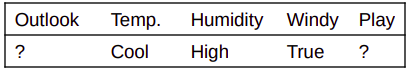
\includegraphics[width=0.45\textwidth]{missingvalue.png}
	\end{figure}
	\item Solution: \textbf{omit} the attribute with missing value in prediction calculation.
	
	$\rightarrow$ take the \textbf{maximum} of $Pr(\text{play} | e_2, e_3,e_4)$ and $Pr(\neg \text{play}|e_2,e_3,e_4)$
\end{itemize}

\subsubsection{Numeric Attributes in Dataset}
\begin{itemize}
	\item Definition: instead of nominal attributes (eg: Outlook = sunny, overcast, cloudy), \textbf{attribute is numeric} (eg: Temperature = 87, 90)
\end{itemize}

\paragraph{Assumption: Attribute Follows Normal Distribution}
\begin{itemize}
	\item Solution:
	\begin{itemize}
		\item Assumption: numeric attributes follows \textbf{normal distribution} $e_i \sim N(\mu,\sigma^2)$
		$$f(x) = \frac{1}{\sqrt{2\pi}\cdot \sigma}\cdot e^{-\frac{(x-\mu)^2}{2 \sigma^2}}$$
		\item calculate the \textbf{mean} and \textbf{standard deviation} for \textbf{each result class}.
		\item conditional probability: \textbf{insert} the numeric instance into the \textbf{probability density function} f(x).
	\end{itemize}
	
	
\end{itemize}

\paragraph{Assumption: Attribute Follows Unknown Distribution}
\begin{itemize}
	\item If the numeric data follows a \textbf{unknown distribution f(x)} (normal distribution not applied) 
	
	$\rightarrow$ probability density distribution \textbf{estimation}.
	\item Solution: kernel density estimation 
	\begin{itemize}
		\item Estimator: Rosenblatt-Parzen Kernel-Density Estimator 
		\item f(x) is not a normal distribution, but each sample follows a normal distribution.
		
		$\rightarrow$ f(x) is the \textbf{sum} of normal distribution at each data point $x_i$
	\end{itemize}
\end{itemize}

\subsection{Prediction using 0-Rule \& 1-Rule}
\begin{itemize}
	\item Input: a dataset $D = x_1, x_2, \dots, x_n$ tuples (evidence, result class), a set of classes $C = C_1, C_2, \dots , C_m$, a \textbf{new instance} with evidence $e_1, \dots, e_k$
	\item Output: classification prediction result 
\end{itemize}
\subsubsection{0-Rule}
Process:
\begin{itemize}
	\item count \textbf{absolute frequency} for each class (classification labels)
	\item Prediction result: class with \textbf{maximum} absolute frequency
\end{itemize}
\subsubsection{1-Rule}
Process:
\begin{itemize}
	\item build \textbf{frequency tables} for each evidence/attribute $e_i$ $\rightarrow$ absolute frequency
	\item pick the \textbf{most frequent class} as classification result for \textbf{each attribute value}
	\item calculate \textbf{overall error rate of the evidence/attribute} according to the classification result
	\begin{figure}[H]
		\centering
		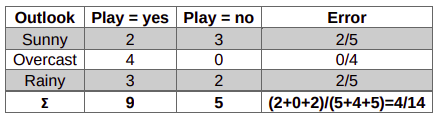
\includegraphics[width=0.45\textwidth]{1-rule.png}
	\end{figure}
	\item Prediction result: choose a \textbf{single attribute} with \textbf{smallest overall error rate}, pick the \textbf{most frequent class} of that evidence/attribute value.
\end{itemize}
Evaluation:
\begin{itemize}
	\item uses only a \textbf{single} attribute for the classification
	\item no prediction result possible if missing value for the attribute found in new instance.
	\item if numeric values in dataset, discretization of the numeric values though possible, but increase the class complexity.
\end{itemize}

\subsection{Prediction using Bayes Theorem: Maximum A Posteriori Classification }
Process:
\begin{itemize}
	\item \textbf{sort} the hypothesis/classification labels, get \textbf{prior probability of hypothesis} $Pr(h), Pr(\neg h)$
	\item  build \textbf{frequency tables} for each evidence/attribute $e_i$ $\rightarrow$ \textbf{absolute frequency}
	\begin{figure}[H]
		\centering
		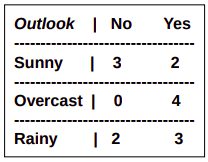
\includegraphics[width=0.25\textwidth]{fre_table.png}
	\end{figure}
	\item check if there is \textbf{zero frequency problem} for the \textbf{attributes from new instance}, resolve by \textbf{adding 1}. 
	
	check for \textbf{numeric} attributes, calculate the \textbf{mean} and \textbf{standard deviation} for each result class.
	\item build \textbf{likelihood tables} for each evidence/attribute $e_i$ $\rightarrow$ \textbf{relative frequency} $Pr(e_i|h)$
	\begin{figure}[H]
		\centering
		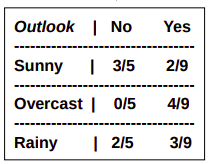
\includegraphics[width=0.25\textwidth]{like_table.png}
	\end{figure}
	\item find $\Pi_{i=1}^k Pr(e_i|h) \cdot Pr(h)$ and $\Pi_{i=1}^k Pr(e_i|\neg h) \cdot Pr(\neg h)$, \textbf{omit} the attribute if \textbf{missing value} in instance.
	\item \textbf{normalize} the result: 
	
	$$Pr(h|e_1,\dots, e_k) = \frac{\Pi_{i=1}^k Pr(e_i|h) \cdot Pr(h)}{Pr(e_1, \dots, e_k)}$$
	$$Pr(\neg h|e_1,\dots, e_k) = \frac{\Pi_{i=1}^k Pr(e_i|\neg h) \cdot Pr(\neg h)}{Pr(e_1, \dots, e_k)}$$ 
	with
	$$Pr(e_1, \dots, e_k) = \Pi_{i=1}^k Pr(e_i|h) \cdot Pr(h) + \Pi_{i=1}^k Pr(e_i|\neg h) \cdot Pr(\neg h)$$

	\item Prediction result: take the \textbf{maximum}.
	$$\text{result} = \max\left\lbrace Pr(h|e_1,\dots, e_k), Pr(\neg h|e_1,\dots, e_k)\right\rbrace $$
\end{itemize}



\subsection{Evaluation of Naive Bayes}
\begin{itemize}
	\item Complexity: 
	\begin{itemize}
		\item calculation of conditional probability: $\mathcal{O}(n)$, 
		
		n: number of instances
		\item calculation of class: $\mathcal{O}(c\cdot p)$, 
		
		c: number of classes, p: number of attributes
	\end{itemize}
	
	\item Advantages: 
	\begin{itemize}
		\item multinomial classification
		\item works well, even if independence assumption is sometimes violated.
	\end{itemize}
	\item Disadvantages:
	\begin{itemize}
		\item takes all attributes with equal weight, could be \textbf{redundant}.
		\item many numeric attributes are actually \textbf{not normally distributed}. 
	\end{itemize}
\end{itemize}

\section{Bayesian Network: Multinomial Classification with Denpendency}

\begin{itemize}
	\item Idea: 
	\begin{itemize}
		\item Naive Bayes assumption too restrictive: \textbf{all} attributes are conditionally independent and equally important.
		\item Attributes are often \textbf{correlated/dependent with each other}
		\item Some attributes are \textbf{redundant} to the classification result.
	\end{itemize}	
	$\rightarrow$ conditional independence among \textbf{subset} of attributes.
\end{itemize}

\subsection{Representation of Bayesian Network: Directed Acyclic Graph}
\begin{itemize}
		\item nodes: attributes
		\item edges: end node is dependent on start node / start node has direct influence on end node.
		\begin{itemize}
			\item start: trigger/cause, evidence node
			\item end: result/effect. 
		\end{itemize}
	\end{itemize}

\begin{figure}[H]
	\centering
	\begin{minipage}{0.5\textwidth}
		\centering
		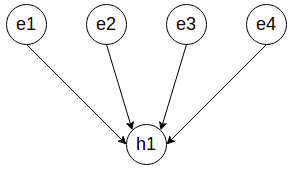
\includegraphics[width=0.45\linewidth]{dag_naivebayes.png}
	\end{minipage}%
	\begin{minipage}{.5\textwidth}
		\centering
		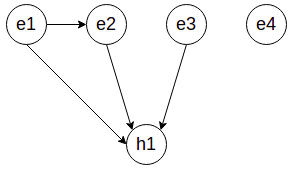
\includegraphics[width=0.45\linewidth]{dag_bayesnet.png}
	\end{minipage}
	\caption{DAG - Naive Bayes(left) vs. Bayesian Network(right)}
\end{figure}
\subsection{Probability Law in Bayesian Network}
\subsubsection{Chain Rule}
According to the \textbf{directed acyclic graph}, derive the \textbf{joint probability distribution} 
	
	$$Pr(e_1, e_2, \dots, e_k) = \Pi_{i=1} Pr(e_i| e_{i-1}, \dots, e_1) = \Pi_{i=1} Pr(e_i| \text{Parents}(e_i))$$
\\ \ \\	
eg: $Pr(A,B,C,D,E) = Pr(A)\cdot Pr(B) \cdot Pr(C|A,B) \cdot Pr(D|A,B,C) \cdot Pr(E|A,C,D)$


\subsubsection{Conditional Independence}
\paragraph{conditional independence between hypothesis and evidence} the hypothesis $h$ is only dependent on $e_1, e_2, e_3$, not on $e_4$ (redundant), then 
	 $$Pr(h | e_1, e_2, e_3, e_4) = Pr(h | e_1, e_2, e_3) $$

\paragraph{conditional independence between hypotheses}

 if two hypotheses are \textbf{independent} from each other, then
	$$Pr(h_1, h_2 | e_1, e_2) = Pr(h_1|e_1,e_2) \cdot Pr(h_2|e_1,e_2)$$

\subsection{Inference in Bayesian Networks}
\begin{itemize}
	\item Idea: infer the probability of an event, given only observation of \textbf{a subset} of other attributes. 
	
	$\rightarrow$ explain the \textbf{away effect} of attributes.
	\item Inference Rules: using \textbf{d-separation}
	\begin{figure}[H]
		\centering
		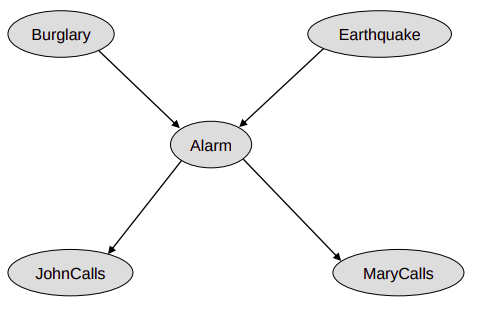
\includegraphics[width=0.4\textwidth]{baynet_example.png}
	\end{figure}
	Example:
	\begin{itemize}
		\item alarm \textbf{not observed}: Burglary \& Mary-calls \textbf{dependent}
				
		$\rightarrow$ if B, belief M $\uparrow$. if M, belief B $\uparrow$.
		
		\item alarm \textbf{observed}: Burglary \& Mary-calls \textbf{conditionally independent}.
				
		$\rightarrow$ no alarm. if Mary-calls, belief B $-$. if B, belief M $-$. 
	\end{itemize}
\end{itemize}

\subsection{Evaluation of a Bayesian Network}
\begin{itemize}
	\item Quality Metrics:
	\begin{itemize}
		\item To maximize the joint probability of training data, the Log-Likelihood of the training data.
		\item Akaike Information Criterion (AIC)
	\end{itemize}
	\item Advantages:
	\begin{itemize}
		\item can handle dependencies among the attributes
	\end{itemize}
	\item Disadvantages:
	\begin{itemize}
		\item computationally expensive, given whether the network structure (DAG) is given, whether the attributes are observable.
	\end{itemize}
\end{itemize}
